\section{相关工作}

\cpar{大型多模态模型。} 一个长期的研究目标是开发能够通过多种模态感知世界的模型,这类似于人类的感官体验。最近,在视觉和语言处理方面的进展使得研究焦点从较小的任务特定模型转向可以处理多种输入的大型通用模型 \citep{team2023gemini,hurst2024gpt4o}。至关重要的是,经过预训练的视觉和语言骨干通常只需很少的适应,就能有效实现跨模态通信 \citep{tsimpoukelli2021multimodalfrozen,shukor2023epalm,vallaeys2024improveddepalm,merullo2023linearly,koh2023grounding}。仅仅将视觉编码器与编码-解码架构 \citep{shukor2023unival,wang2022ofa,lu2022unified,mizrahi20234m} 或解码器-only LLM 结合,就能构建出功能强大的多模态系统 \citep{laurenccon2024mattersidefics2,alayrac2022flamingo,liu2024improvedllava,wang2024qwen2,xue2024xgenblip3,chen2024internvl,zhu2024minigpt,abdin2024phi3,dai2024nvlm,beyer2024paligemma,moon2024anymal}。这种后融合方法,在模态先分别处理再结合的过程中,现已得到充分理解,并且有了训练有效模型的最佳实践 \citep{laurenccon2024obelics,mckinzie2025mm1,zhang2024mm1_5,lin2024vila}。相比之下,早期融合模型 \citep{fuyu8b,team2024chameleon,diao2024unveiling},即在更早阶段就将模态结合,仍然相对较少被探索,只有有限数量的公开发布模型 \citep{fuyu8b,diao2024unveiling}。与 \citep{diao2024unveiling,team2024chameleon} 不同,我们的模型仅使用一个线性层,并完全依赖于下一个令牌预测损失。此外,我们的模型从零开始训练所有模态,而无需图像标记化。

\cpar{原生多模态模型。} 我们将原生多模态模型定义为那些同时从零开始在所有模态上进行训练的模型 \citep{team2023gemini},而不是将LLM适配到其他模态。由于训练此类模型的成本很高,它们仍然相对未被深入研究,大多数模型依赖于后融合架构 \citep{kosmoshuang2023language,yu2022coca}。一些从零开始训练的多模态模型 \citep{aghajanyan2022cm3,team2024chameleon,wang2024emu3} 通过使用如 \citep{vqgan,vqvae} 这样的预训练图像标记器,将图像转换为离散令牌,并将其集成到文本词汇中,从而放宽了这一约束。这种方法使得模型能够理解并生成文本和图像,促进了更顺畅的多模态学习过程。

\cpar{扩展定律。} 扩展定律研究旨在预测模型性能如何随着训练计算资源的增加而变化。早期的研究 \citep{kaplan2020scaling,hoffmann2022training} 发现,LLM性能与计算资源呈幂律关系,这使得能够基于计算资源预算来估算模型参数数量和训练令牌数量的计算最优值。类似的研究将这些发现扩展到了稀疏专家混合(MoE)模型,考虑了稀疏性、专家数量和路由粒度等因素 \citep{krajewski2024scalingmoe,clark2022unifiedscalingmoe,wangscalingmoe}。扩展定律还在多个领域得到了观察,包括图像模型 \citep{fini2024multimodalaimv2}、视频模型 \citep{rajasegaran2025empirical}、蛋白质LLM \citep{scalingprotein} 和模仿学习 \citep{pearce2024scaling}。然而,关于多模态模型的扩展定律的研究较少。特别是,\citet{aghajanyan2023scalingmm} 考察了将模态标记为离散令牌并包括多模态生成的多模态模型。相比之下,我们重点研究的是早期融合模型,它们接受原始多模态输入,并在交错的多模态数据上进行训练。

\cpar{专家混合(MoEs)。} 专家混合(MoE) \citep{shazeer2017outrageously} 通过将模型容量与每个样本的计算资源解耦,能够扩展模型容量。这是通过稀疏激活少量参数来实现的。这种方法使得大型稀疏模型能够与密集模型竞争,同时在训练和推理过程中更为高效 \citep{fedus2022switch,sun2024hunyuan,jiang2024mixtral,liu2024deepseekv3,wei2024skywork}。许多研究探讨了改进MoE LLM的各个方面,如负载平衡、路由、稳定性、扩展性和粒度 \citep{lewis2021base,zoph2022st,lepikhin2020gshard}。然而,对于将MoE应用于多模态模型的研究较为有限,一些工作集中在对比图像-文本模型 \citep{mustafa2022multimodal} 和后融合多模态LLM \citep{lin2024moe,li2024aria} 上。此外,一些研究探讨了预定义的专家路由,其中某些参数专门处理特定的模态 \citep{bao2021vlmo,chen2024eve,shen2023scaling}。我们专注于研究MoE在原生早期融合模型中的应用,而不是提出新的架构。



\begin{figure}[t!]
    \centering
    \captionsetup{type=figure}
    \begin{subfigure}[h]{0.95\linewidth}
    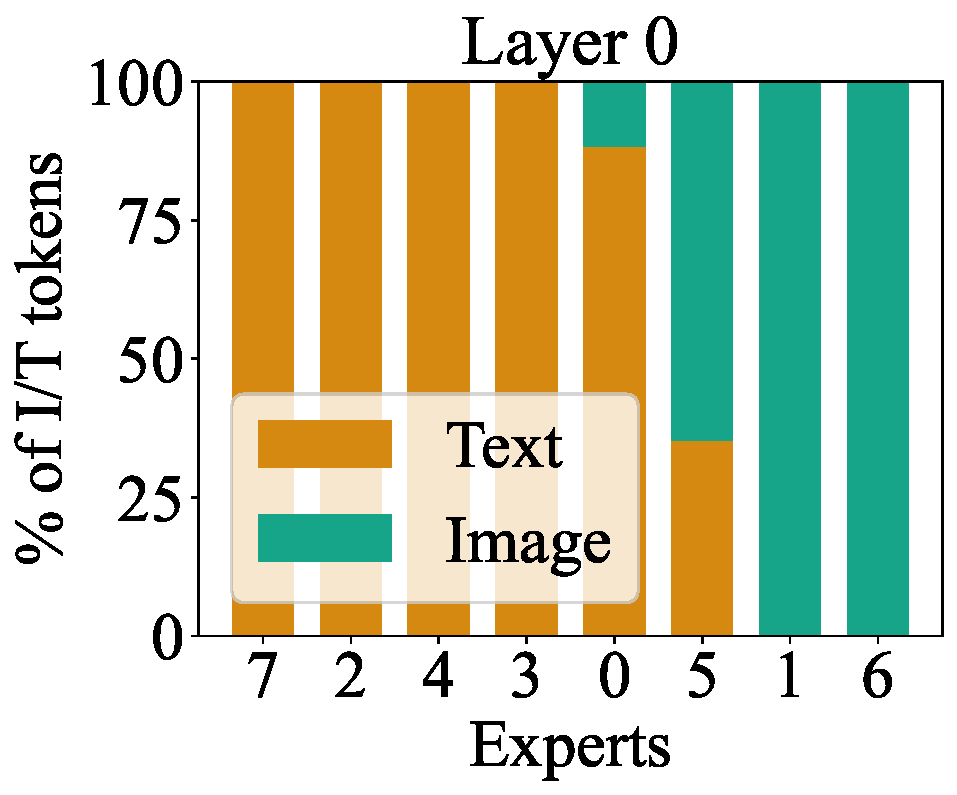
\includegraphics[height=0.27\textwidth]{assets/moes/specialization/sorted/tokens_assignment_obelics_1088_150_0.pdf}
    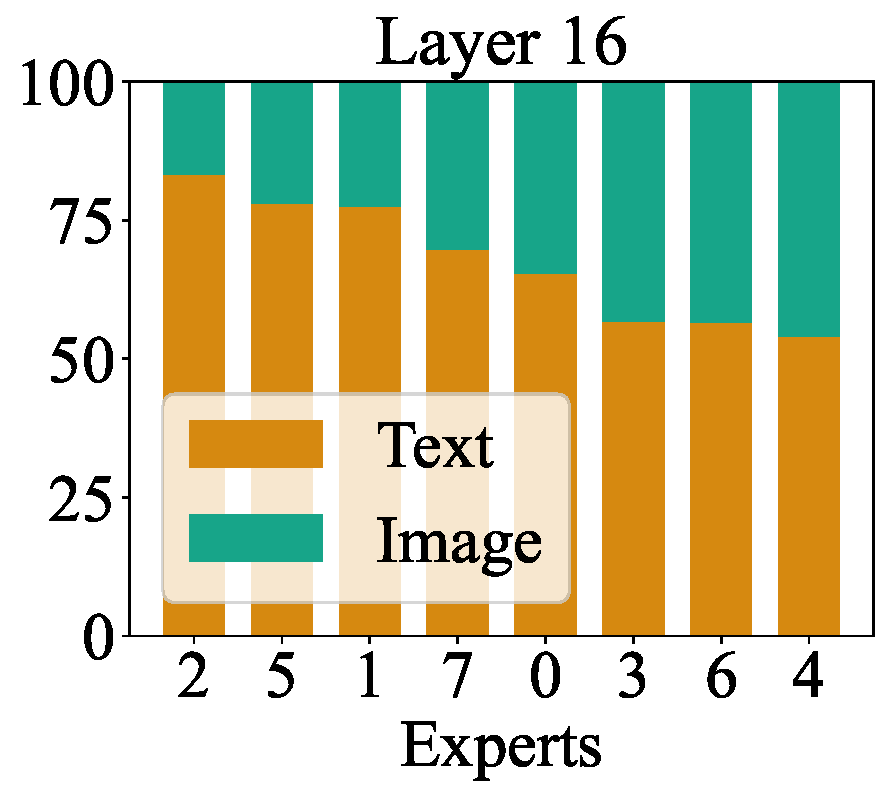
\includegraphics[height=0.27\textwidth]{assets/moes/specialization/sorted/tokens_assignment_obelics_1088_150_16.pdf}
    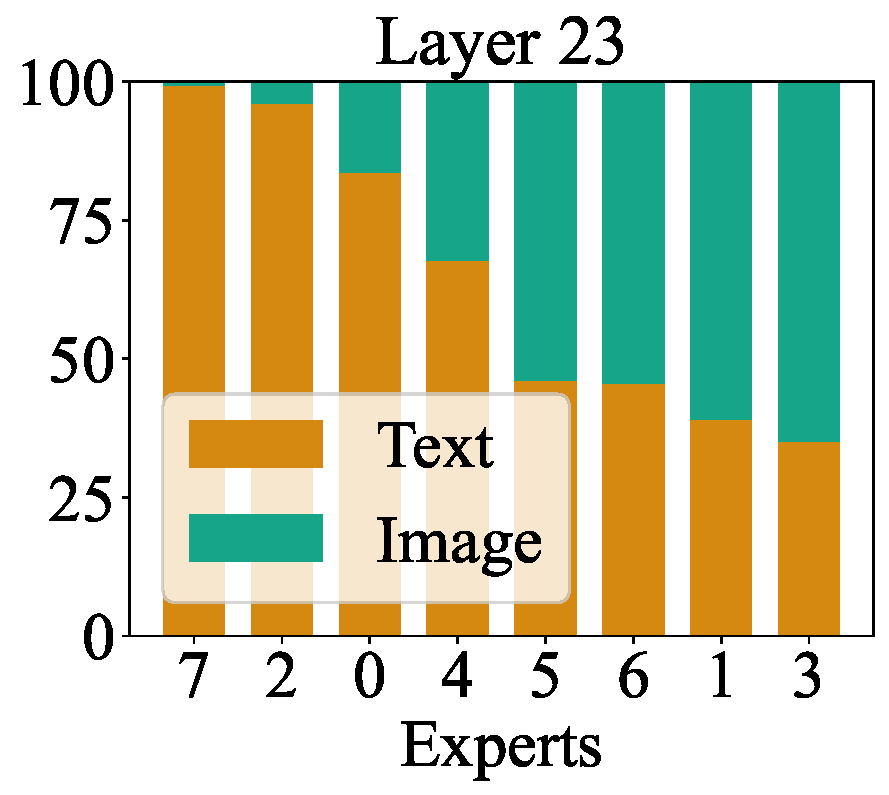
\includegraphics[height=0.27\textwidth]{assets/moes/specialization/sorted/tokens_assignment_obelics_1088_150_23.pdf}
    \end{subfigure}    \caption{\textbf{MoE 特化频率。} 从 Obelics 的交错数据中,路由到每个专家的文本和图像词元的百分比。专家按顺序排列以获得更好的可视化效果。第一层显示了最多的单峰值专家。}
    \label{fig:tokens_assignment}
\end{figure}

